\documentclass[final]{beamer}
\usetheme{posterstyle}
\usepackage[absolute,overlay]{textpos}
\usepackage[orientation=portrait,scale=1.35]{beamerposter}
\usepackage{cutwin}
\newlength{\sepwid}  
\newlength{\onecolwid}  
\newlength{\twocolwid}  
\newlength{\threecolwid}  
\setlength{\paperwidth}{24in}  
\setlength{\paperheight}{36in}    
\setlength{\sepwid}{0.025\paperwidth}
\setlength{\onecolwid}{0.21875\paperwidth}
\setlength{\twocolwid}{0.4625\paperwidth}
\setlength{\threecolwid}{0.70625\paperwidth}
\setlength{\topmargin}{-1in}
\setlength{\TPHorizModule}{1in}
\setlength{\TPVertModule}{1in}
\setlength{\leftmargini}{1in}
\setlength{\itemsep}{9in}

\title{Predicting Chronic Diseases with Machine Learning}
\author{Vlad Korolev}
\date[]{ \today}
\footer{Work in progress \hskip 0.72\textwidth  ebiquity.org}

\begin{document}


\begin{frame}{} 
\begin{textblock}{23.5}(.2,1.75)
\begin{block}{\center Focus \vskip .2in}
\begin{enumerate}
\item Use machine learning techniques aid in determining predisposition to chronic decease based on individual's genetic information and clinical data.   
\item \alert{Use all available data from SNP profile}
\end{enumerate}
\end{block}
\end{textblock}

\begin{textblock}{23.5}(.2,5.52)
\begin{block}{\center Genetic Causes of Chronic Diseases}
\end{block}
\end{textblock}

\begin{textblock}{6,8}(.2,6.5)
\begin{block}{}
\vskip .25in
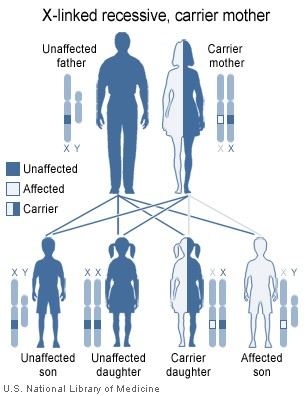
\includegraphics[width=6in,height=7.25in]{XlinkRecessive.jpg}
\vskip 1.5in
\end{block}
\end{textblock}


\begin{textblock}{8}(7.25,6.5)
\begin{block}{}
\vskip .25in
\begin{center}
{\bf  Single Gene Disorders}
\end{center}
\vskip .25in
\begin{itemize}
\item <1->Depend on a single-gene mutation
\item <1->Have been suspected for long time
\item <1->Have been proven for quite some time
\item <1->Notable examples
    \begin{itemize}
       	\item Sickle cell anemia
	\item Cystic fibrosis
	\item Hemophilia
    \end{itemize}
\item  <1->Easily determined by Mendelian methods, looking at family history
\end{itemize}
\vskip 0.25in
\end{block}
\end{textblock}

\begin{textblock}{8.7}(15,6.5)
\begin{block}{}
\vskip .25in

\begin{center}
{\bf   Multi Gene Disorders}
\end{center}

\begin{itemize}
\item <1->Depend on two or more mutations
\item <1->Well studied mutation : Horse color
\item <1-> Two gene conditions
    \begin{itemize}
       	\item Lactose intolerance
    \end{itemize}
\item <1-> Polygenic complex mutations
\begin{itemize}
\item Asthma
\item Diabetes
\item Cancers
\item Hypertension
\item Autoimmune diseases such as multiple sclerosis
\end{itemize}
\item <1-> Very hard to determine through Mendelian methods
\item <1-> Suspected to be genetic based on tendencies to run in families
\item <1-> No clear pattern of inheritance
\end{itemize}
\end{block}
\end{textblock}

\begin{textblock}{23}(.2,16.9)
\begin{block}{\vskip 1in}
\end{block}
\end{textblock}


\begin{textblock}{8.1}(.2,16.9)

\begin{block}{\center Previous Work \vskip .28in}

\begin{small}
\begin{enumerate}
\item de Miguel-Yanes JM, Shrader P, Pencina MJ, Fox CS, Manning AK, Grant RW. Genetic risk reclassification for type 2 diabetes by age below or above 50 years using 40 type 2 diabetes risk single nucleotide polymorphisms. Diabetes Care. 2011 Jan;34(1):121-5.
\item Lanktree M, Oh J, Hegele RA. Genetic testing for atherosclerosis risk: inevitability or pipe dream? Can J Cardiol. 2008 Nov;24(11):851-4.
\end{enumerate}
\end{small}
\end{block}



\begin{itemize}
\item <1-> Combine clinical and genetic information
\item <1-> Used statistical models
\item <1-> Did not show benefit when including genetic information 

\end{itemize}

\begin{center}{\bf Darshana Delvi, Aniket Bochare} \end{center}

\begin{itemize}

\item<1-> Extracted subset of SNPs that are known to cause the disease

\item<1-> Combined SNPs with clinical data

\item<1-> Trained decision tree algorithm to build a classifier

\item<1-> Cross-validated the classifier to obtain accuracy of the method

\item<1-> \alert{Showed slight improvement over pure statistical methods.  But amount of improvement was not that great.}

\end{itemize}


\end{textblock}



\begin{textblock}{6.75}(8.7,16.9)
\vskip .05in
\begin{block}{\center  Approach \vskip .15in }
\begin{center}{\bf Challenges}\end{center}
\begin{itemize}

\item Large Datasets ( 500 GB )
\item Too many attributes
\item Repeatability of experiments \end{itemize}

\vskip .2in
\begin{center}{\bf Method}\end{center}
\vskip .5in
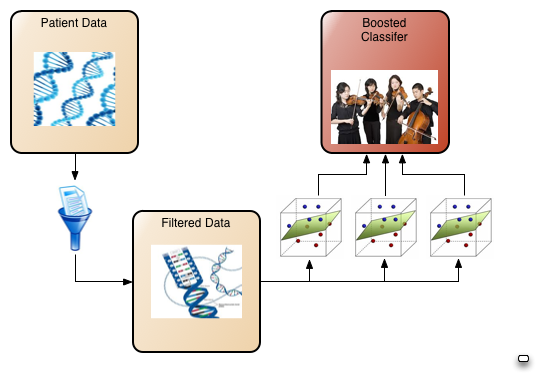
\includegraphics[width=6in]{BuildBoostClassifier4.png}

\vskip .2in

\begin{center}{\bf Objectives}
\vskip .2in
\begin{tabular}{c c}
Capacity & Performance \\
Repeatability & Automation \\
\end{tabular}
\end{center}


\vskip .3in
\center{\bf Platform}\vskip .2in
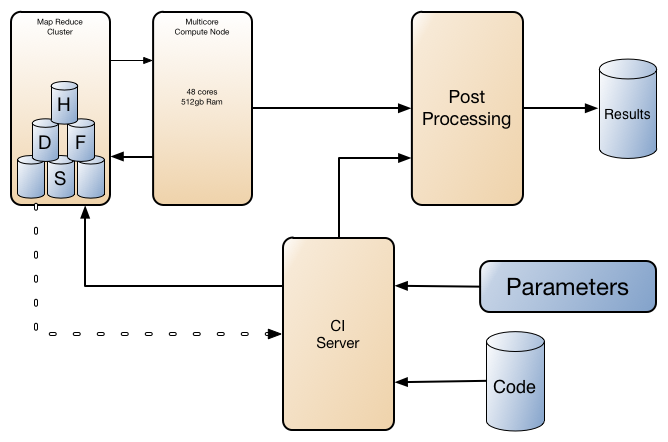
\includegraphics[width=6in,height=4.25in]{Platform1.png}



\end{block}
\end{textblock}


\begin{textblock}{8}(15.7,16.9)
\begin{block}{ \center Initial Results \vskip .3in }
 
 


\vskip .2in



\begin{center}{\bf Prostate Cancer Study }\end{center}

\vskip .2in

\begin{columns}
\column{1in}
	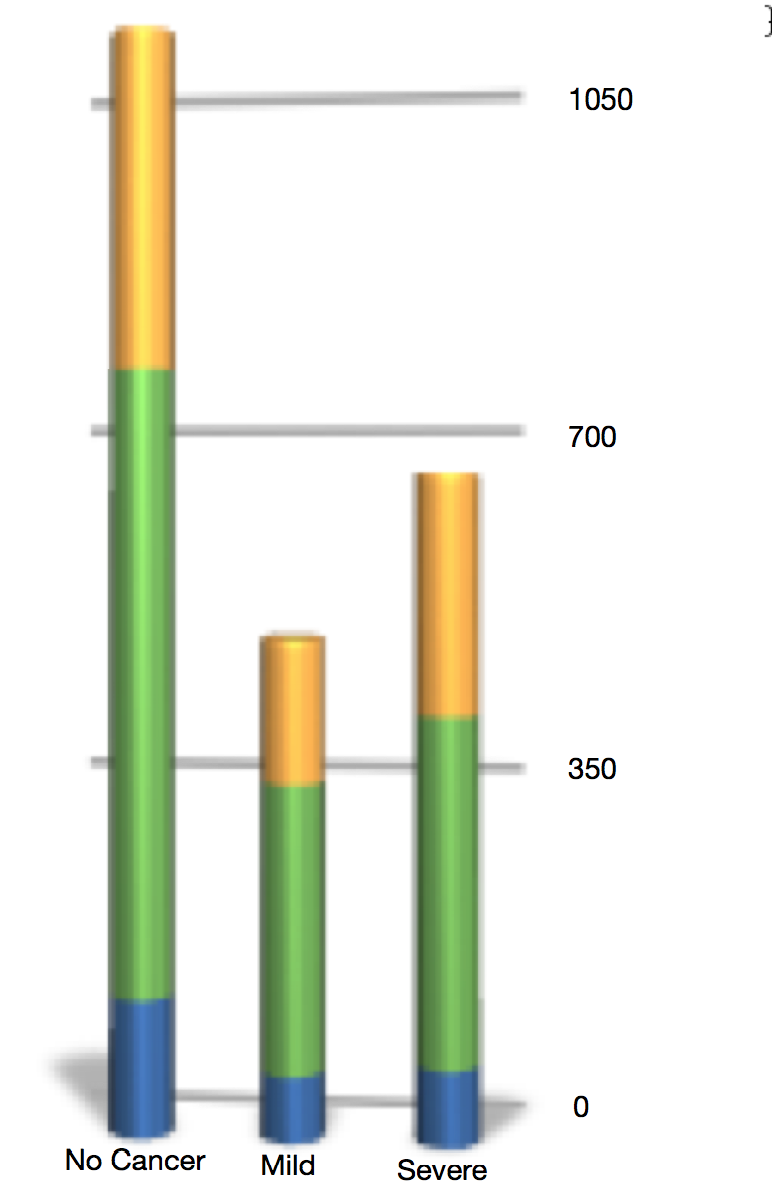
\includegraphics[width=2in,height=3in]{ProstatePopulationBreakdown.png} 	
\column{1in}
\begin{tiny}
\begin{tabular}{l c}
\hline
No Cancer & 1098 \\
Cancer       &  1147 \\
\hline
\end{tabular}
\end{tiny}
\end{columns}

\vskip .2in

\begin{center}{\tiny Combined Feature Frequency}\end{center}


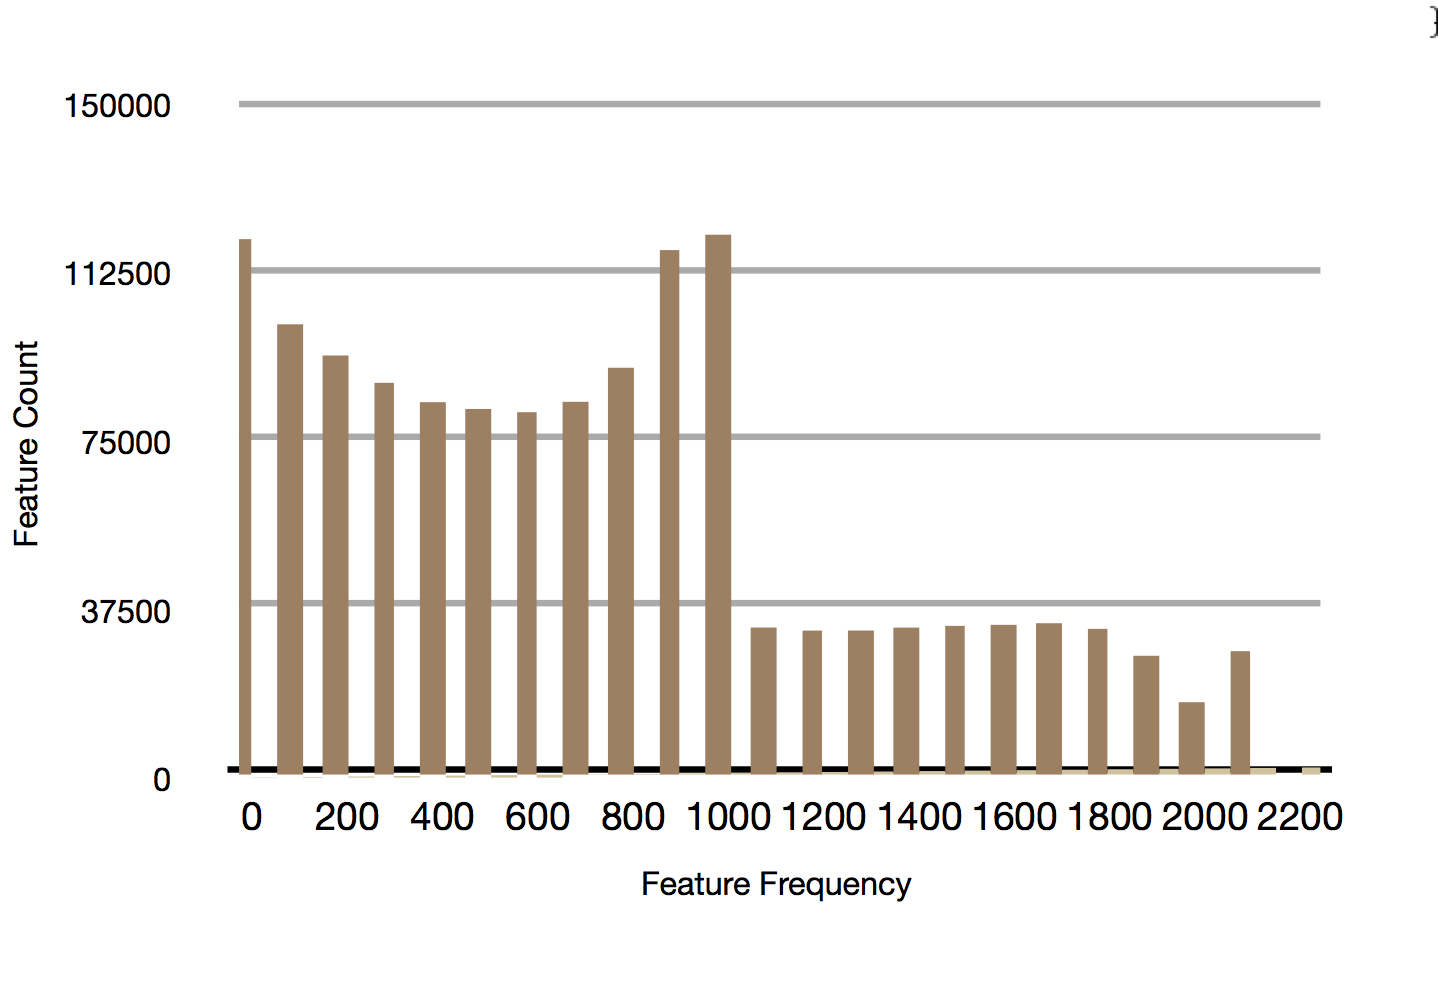
\includegraphics[width=3in]{CombinedFeatureFrequency.png} \hskip 1in
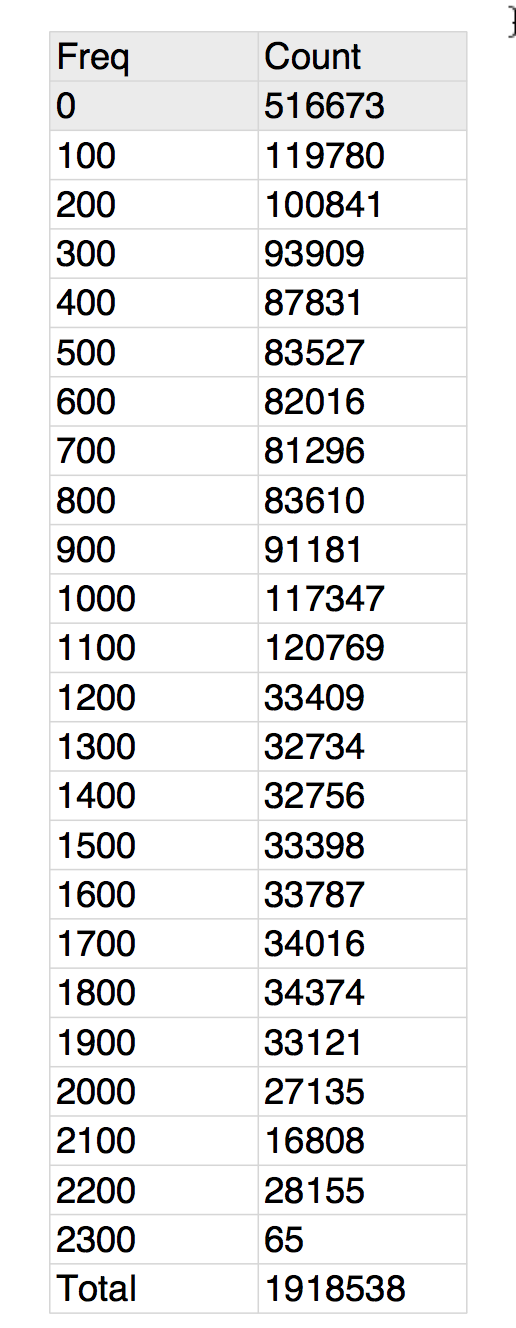
\includegraphics[width=1.5in, height=3in]{FreqTableCombined.png}


\begin{center}{\tiny Feature Frequency : Controls}\end{center}

\begin{columns}
\column{5.75in}
	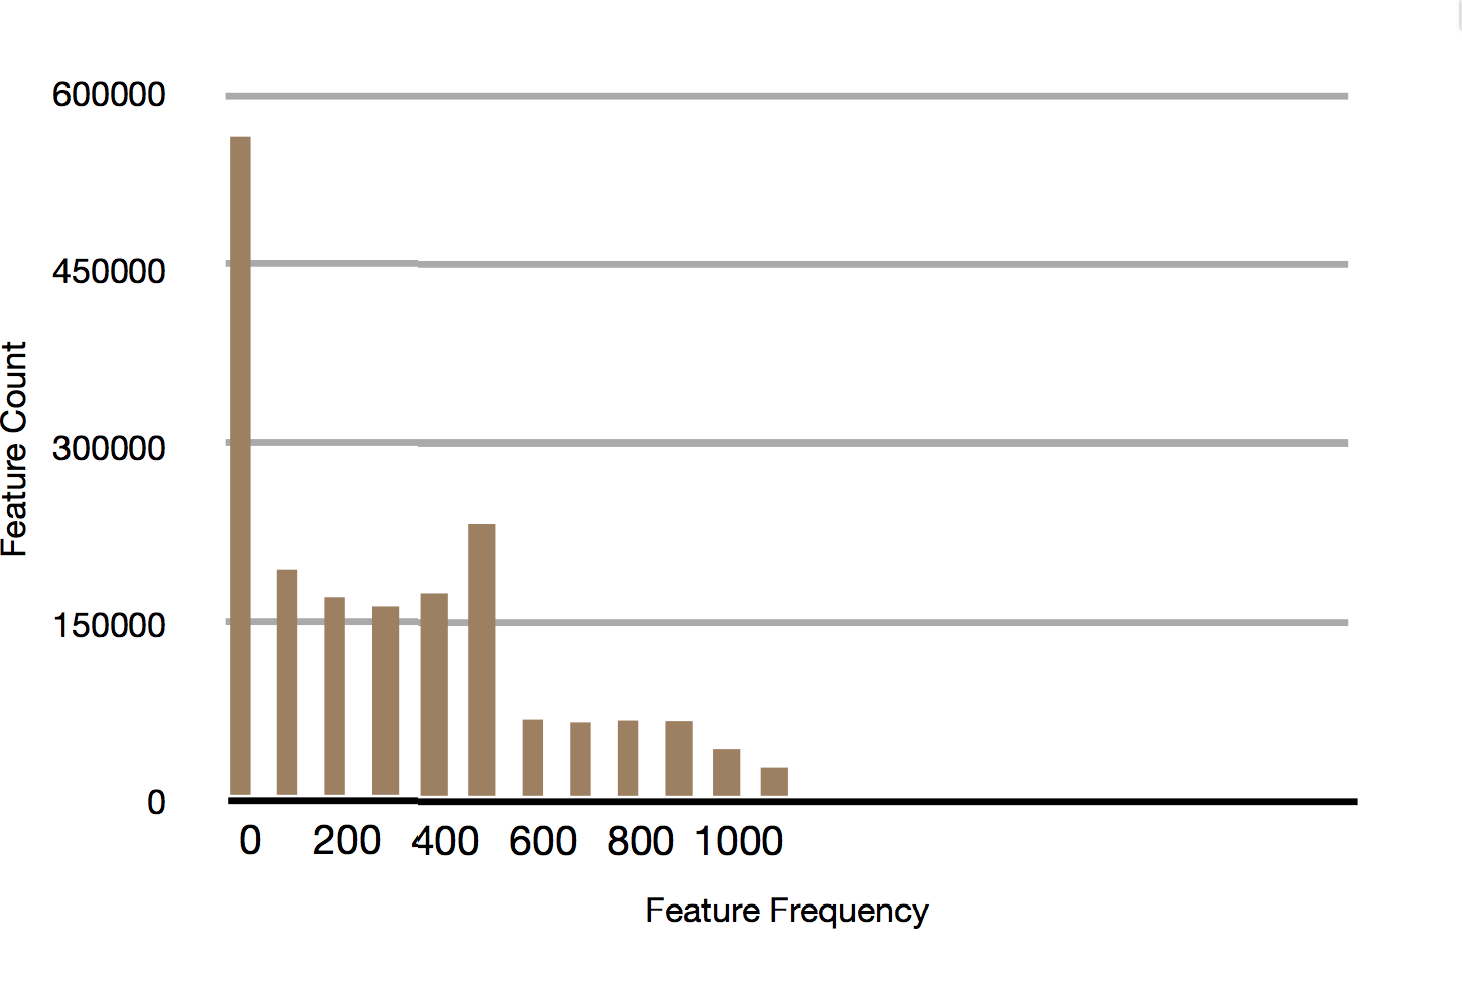
\includegraphics[width=3in,height=2in]{FeatureFrequencyControls.png} 	
	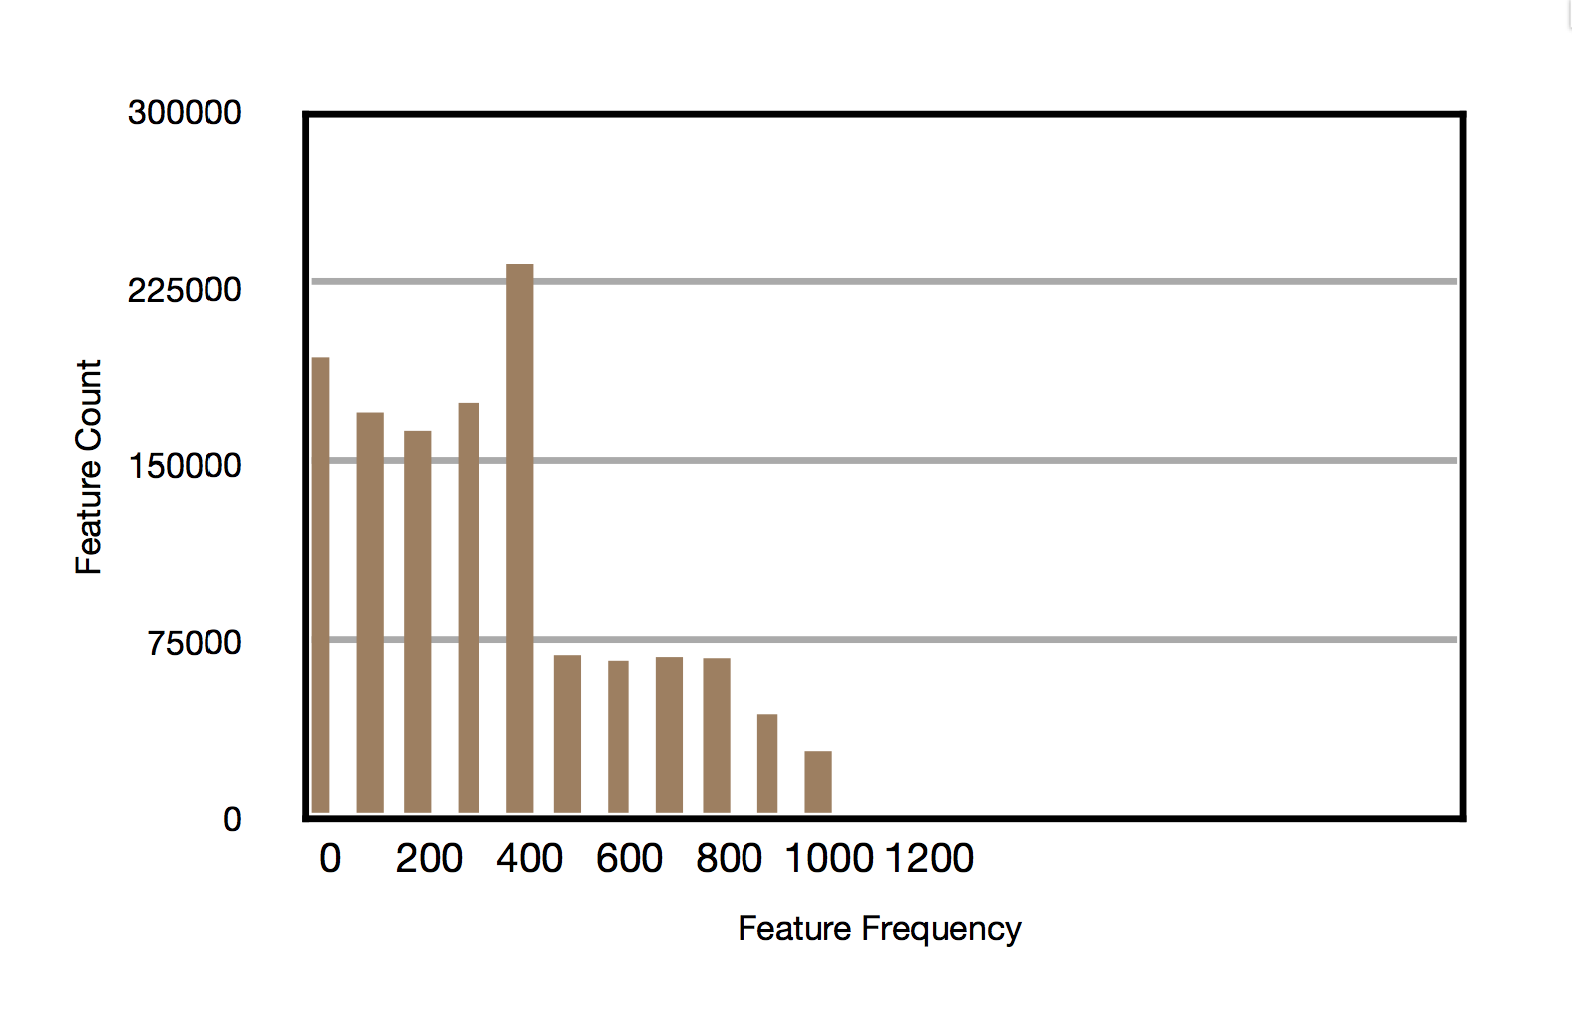
\includegraphics[width=3in,height=2in]{FeatureFrequencyControlsHiPass.png} 	
\column{1in}
	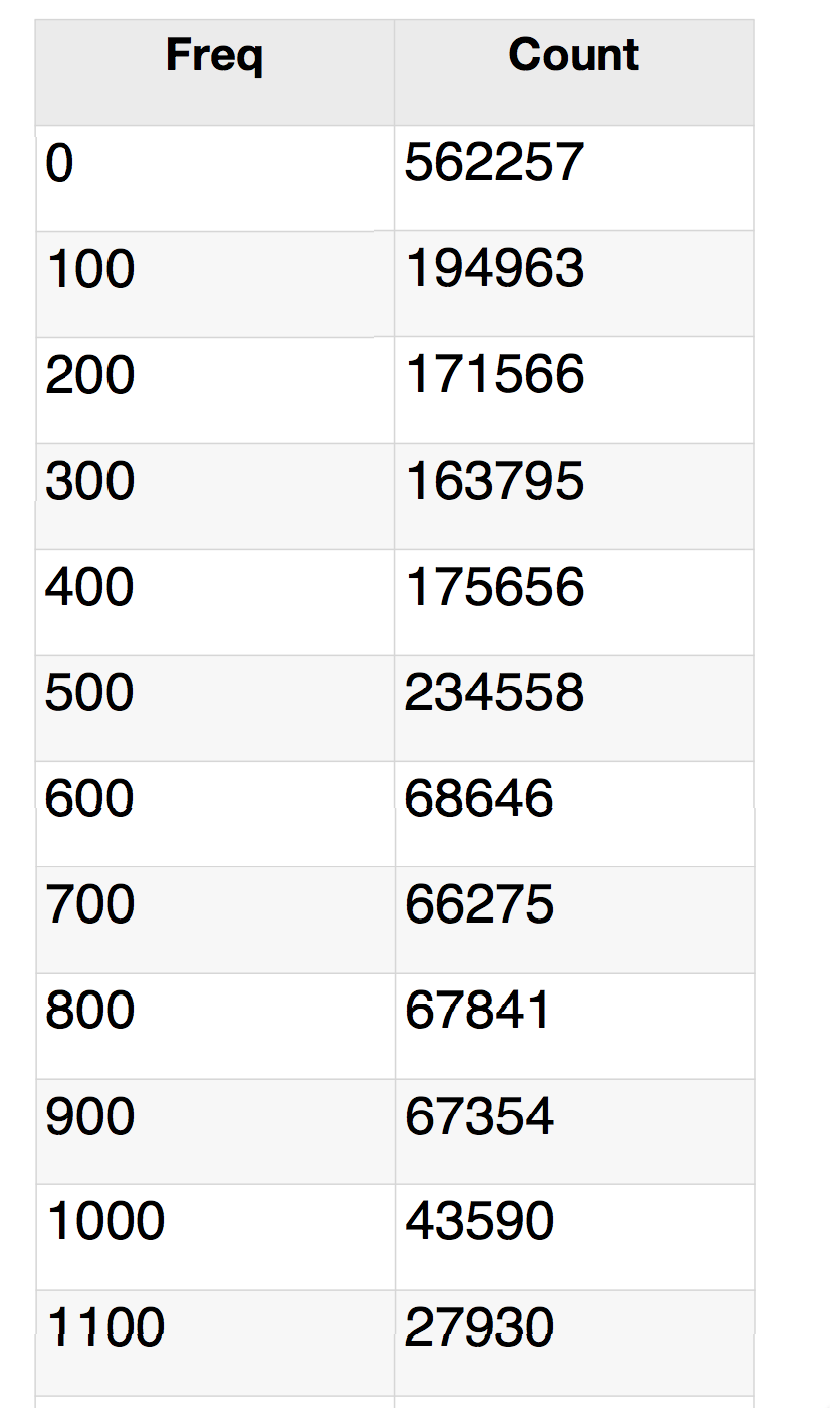
\includegraphics[width=1in]{FreqTableControls.png}
\end{columns}


\begin{center}{\tiny Feature Frequency : Cases}\end{center}

\begin{columns}
\column{6in}
	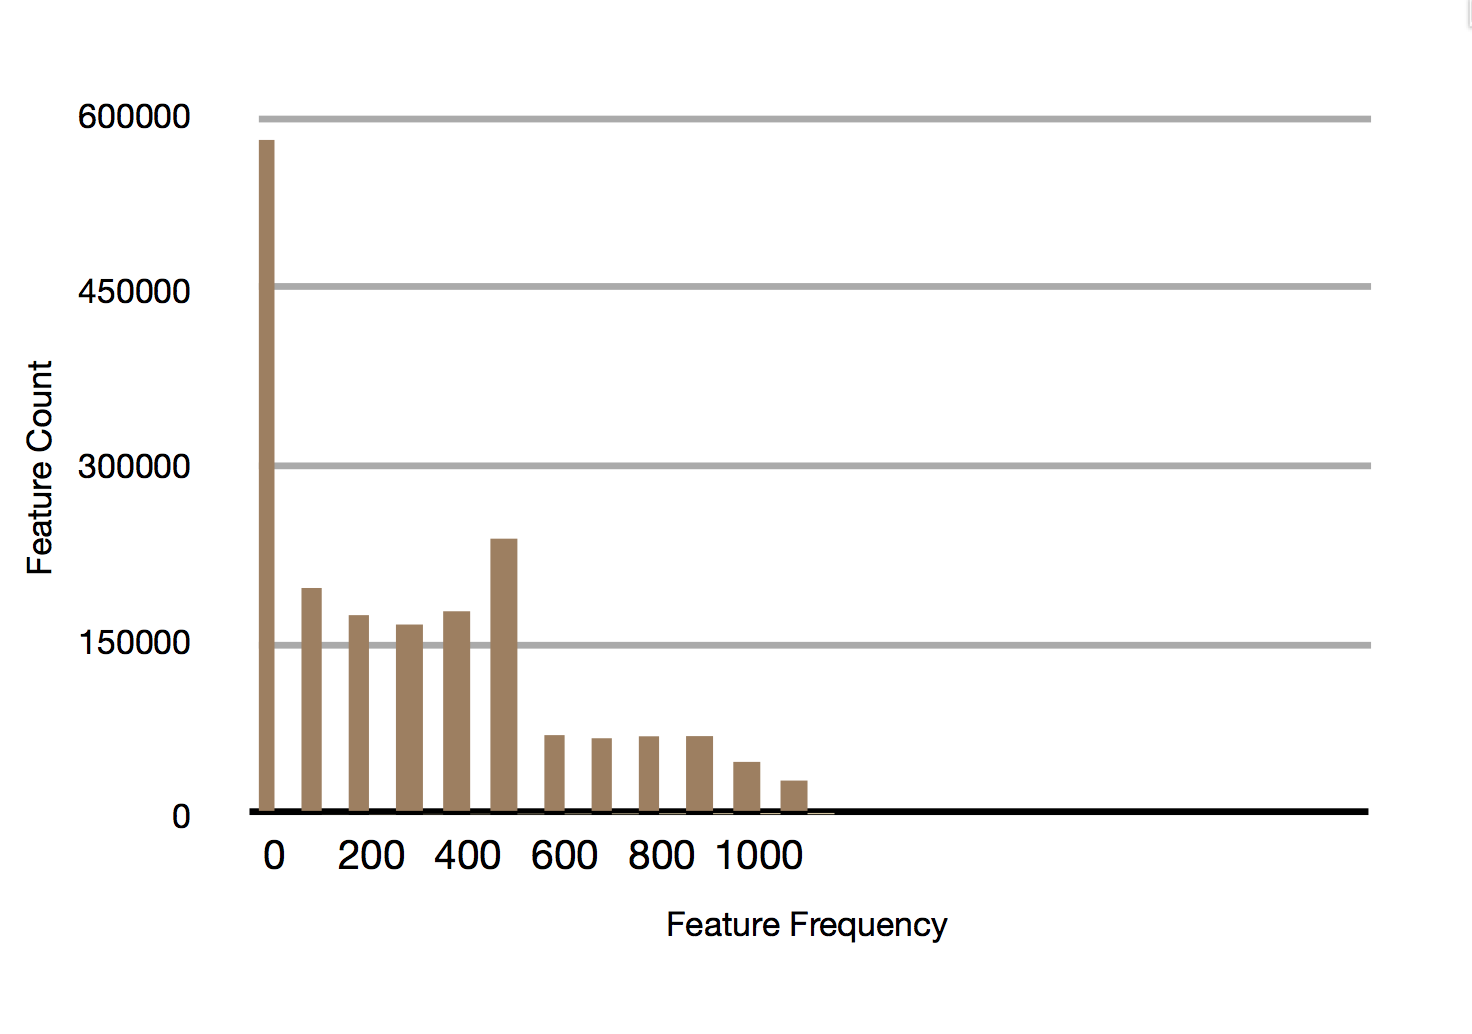
\includegraphics[width=3in,height=2in]{FeatureFrequencyCases.png} 
	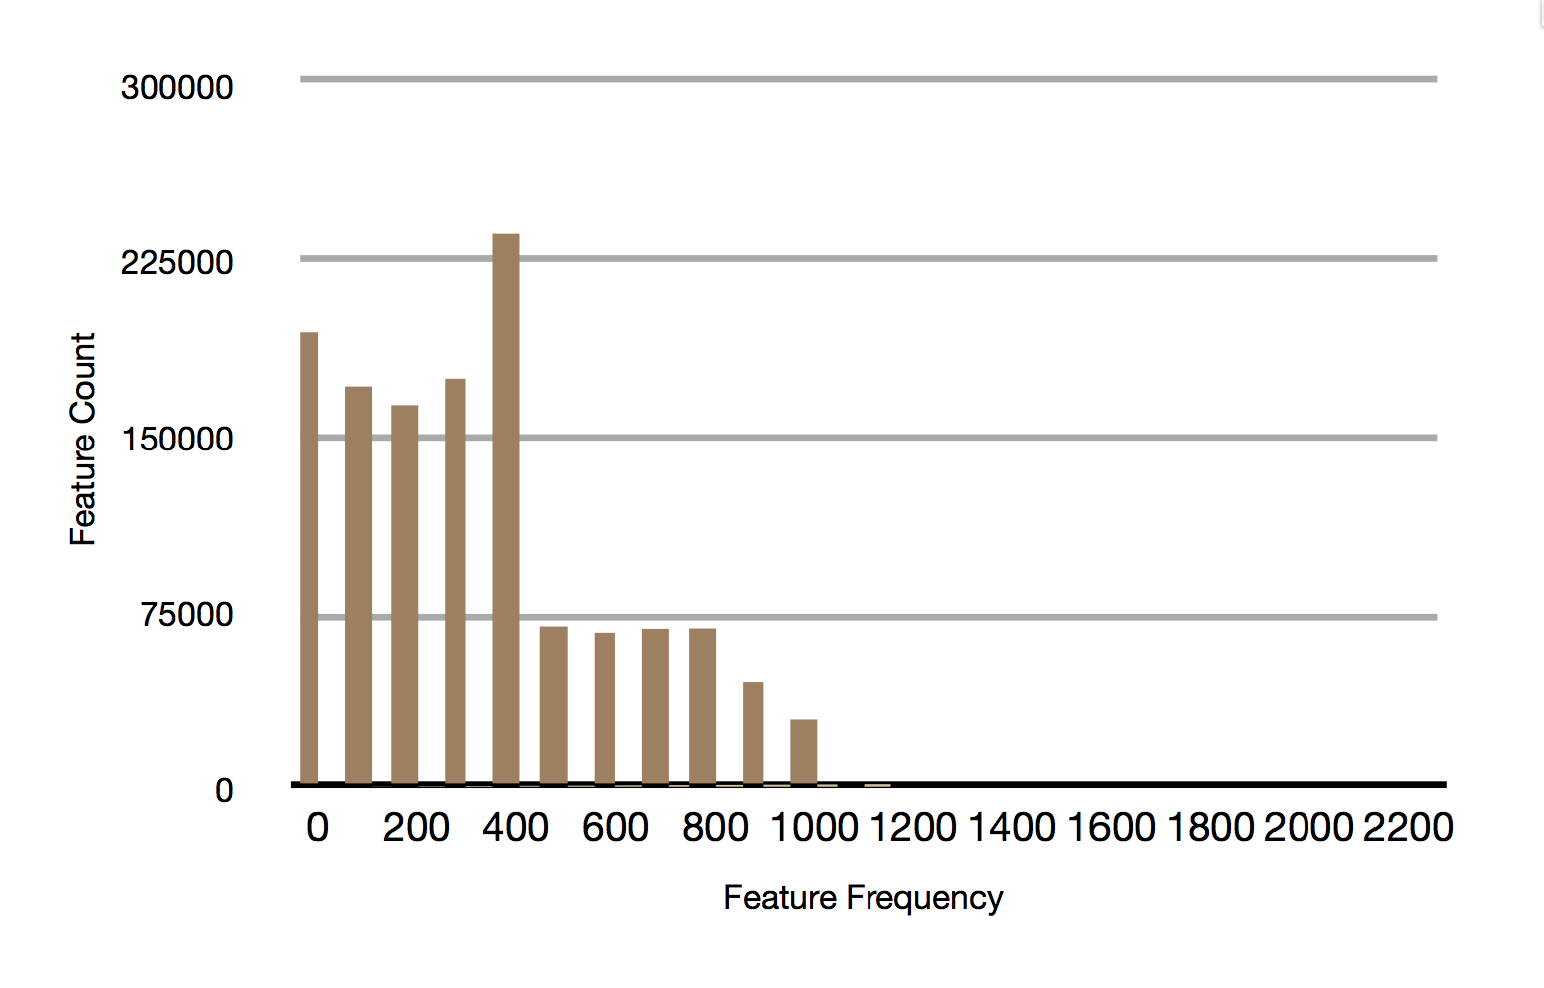
\includegraphics[width=3in,height=2in]{FeatureFrequencyCasesHiPass.png} 

\column{1in}
	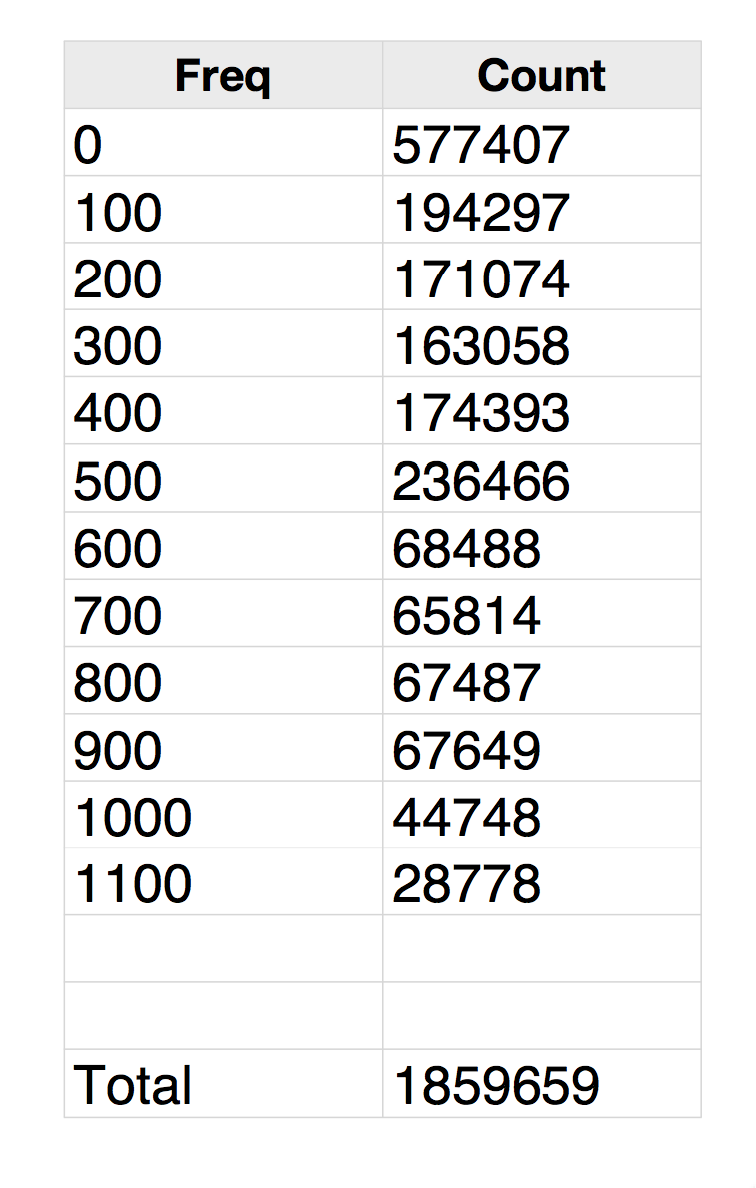
\includegraphics[width=1in]{FreqTableCases.png}
\end{columns}



\end{block}
\end{textblock}





\end{frame}
\end{document}